\documentclass[12pt,a4paper]{scrreprt}
%\documentclass[12pt,a4paper]{report}
\usepackage{CJK,CJKnumb}
\usepackage{indentfirst}
\usepackage{makeidx}
\usepackage{graphicx}
\usepackage{multirow}
\usepackage{syntonly}
\syntaxonly
\newcommand{\tabincell}[2]{\begin{tabular}{@{}#1@{}}#2\end{tabular}}

\graphicspath{{Figure/}}
\makeindex
\setlength{\parindent}{2em}

\begin{document}             % End of preamble and beginning of text.

\begin{CJK*}{UTF8}{gbsn}
%\begin{CJK*}{GBK}{song}
%\CJKcaption{GBK}
%\CJKindent
                             % The preamble begins here.
\title{A Study of Fission Products in the Molten-Salt Reactor Experiment by $\gamma$\ Spectrometry}  % Declares the document's title.
\subtitle{通过$\gamma$\ 谱测量法研究MSRE中的裂变产物}
\author{A. Houtzeel \and F.  F. Dyer}      % Declares the author's name.
\date{August  1972}      % Deleting this command produces today's date.

\maketitle                   % Produces the title.
\renewcommand\abstractname{摘~要}
%\renewcommand\abstractname{摘~要}
\begin{abstract}

熔盐堆实验(MSRE)的运行证实了在反应堆候选者中氟盐混合物作为实际的流体核燃料是相当稳定的。%
然而,有些裂变产物化学物质离开了核燃料\index{核燃料}的循环系统,出现在堆芯石墨慢化剂、和熔盐接触的金属组件表面、排气系统的金属组件表面。%
Xe和Kr裂变气体在排气系统里衰变成其他子体,并被分离出来。%
有些元素(Mo,Nb,Ru,Te,Sb)以金属形式存在,并附着在金属组件表面、石墨表面、或者以粒子的形式被带到排气系统。%
在设计更大的熔盐堆系统中,已知裂变产物以多少比例分布在哪些部位是相当重要的,从MSRE实验中获得信息,并制定出值得考虑的影响因素。

在MSRE实验中,通过测量发射出的 \(\gamma\) 射线的强度和能谱,ORNL发展了一种技术来定位、测量与熔盐接触的表面或排气系统中的裂变产物的沉积情况。%
发展出来的\(\gamma\)谱测量装置包括一个Ge(Li)探头,4096道的多道分析器,和一个用来测量小区域的铅准直器。%
这套装置经常安装在MSRE可移动的维护屏上面,这些维护屏覆盖在堆系统组件的各个部位,通过激光束配合观察员的搬运,可以实现装置的精确准直和固定。

本实验不仅在停堆和排出熔盐时,也在核燃料循环和堆运行在不同功率等级下做测量。总共记录1000多个谱,其中,堆运行在不同功率等级下的记录的谱占了25\%。%
另外,有400个谱用于刻度仪器。计算机化数据处理实现了高质量、大批量的数据的分析能力。

本实验主要的精力集中在排气系统和主热交换器,其中,后者有40\%的金属表面与熔盐接触。%
排气系统不仅包含了气态裂变产物及其母体,还包括金属元素及其衰变产物(例如,Nb,Mo,Ru,Sb,Te(I))。%
MSRE的热交换器主要沉积类似的金属元素。%
当停堆且立即排出燃料(紧急排放)时,实验观察到热交换器的放射性主要来源于裂变气体。

在高放射性堆系统中定位和评估裂变产物的沉积情况,使用了远程维护设备和定位工具的高分辨率$\gamma$射线谱测量法被证实是非常有用的。

\end{abstract}
%插入摘要

\renewcommand\contentsname{目~录}
\tableofcontents

\chapter{MSRE简介}

\section{熔盐堆概念}

\section{MSRE描述}

\begin{figure}
%\graphicspath{{Figure/}}
\centering
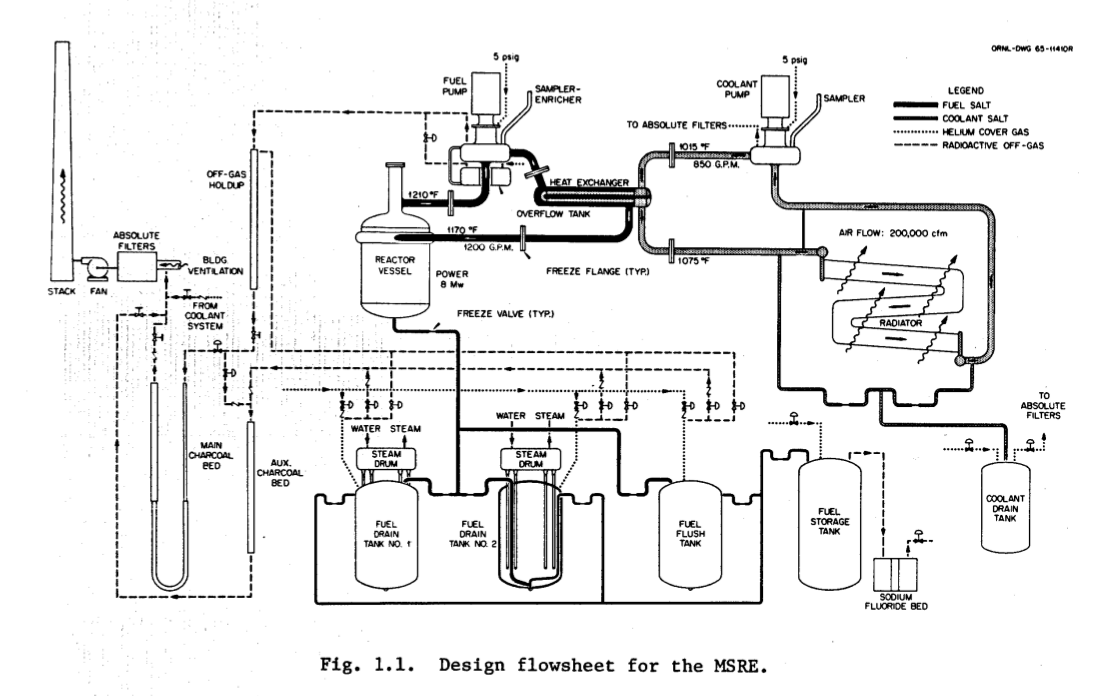
\includegraphics[width=0.8\textwidth]{Fig_1_1}
\caption{Design flowsheet for the MSRE.}
\label{Fig_1_1}
\end{figure}

\begin{figure}
%\graphicspath{{Figure/}}
\centering
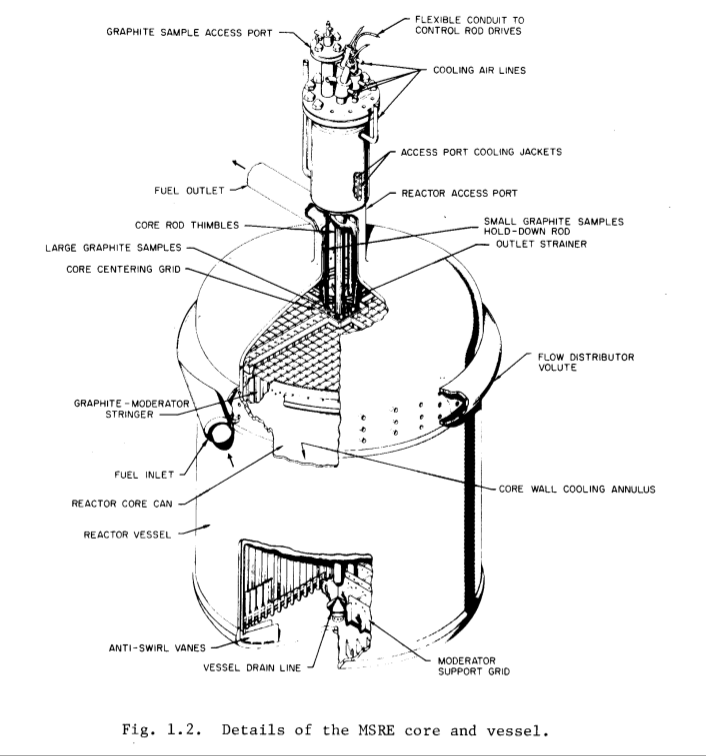
\includegraphics[width=0.8\textwidth]{Fig_1_2}
\caption{Details of the MSRE core and vessel.}
\label{Fig_1_2}
\end{figure}

\begin{figure}
%\graphicspath{{Figure/}}
\centering
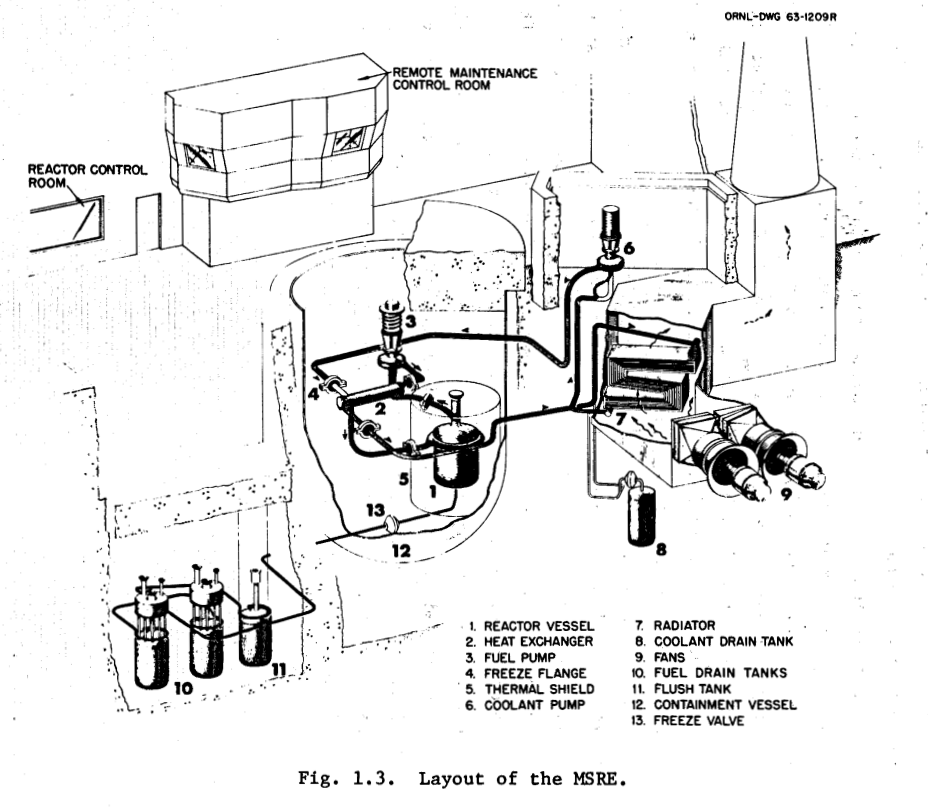
\includegraphics[width=0.8\textwidth]{Fig_1_3}
\caption{Layout of the MSRE.}
\label{Fig_1_3}
\end{figure}
%Introduction to the molten salt reactor experiment
\chapter{研究γ谱测量法的目的}
MSRE的运行证明了氟盐混合物在堆中是稳定的,且大部分裂变产物都保持在循环的核燃料盐中;然而,在堆芯石墨慢化剂、与熔盐接触的金属组件表面和堆排气系统中发现了一些裂变产物。例如,Mo、Nb、Ru、Te、Sb等元素以金属单质的形式存在,并逐渐附着在与熔盐接触的组件上面,或以粒子形式被携带到排气系统中。

在熔盐系统中,某些裂变产物(特别是易挥发或易沉积的)的行为由于以下几个原因而被受关注:
\begin{enumerate}
\item 为了了解熔盐中裂变产物的化学性质。
\item 堆组件的远程维护所需的屏蔽由大量沉积在这些组件上的高放射性裂变产物决定。
\item 对于一个高功率的熔盐堆而言,在停堆和排出燃料之后,冷却这些沉积的裂变产物所释放的几兆瓦特的衰变热将是一个麻烦。
\item 沉积堆积在堆芯石墨里的裂变产物将吸收更多的中子,因此降低熔盐堆的增值性能。
\end{enumerate}
由以上原因,MSRE承担了裂变产物行为研究的整个计划。这篇报告要描述的研究目的是通过远程 $\gamma$ 能谱测量技术对沉积在某些MSRE组件上的放射性裂变产物进行定性、定量测量。尤其关注反应堆的排气系统和热交换器,其中热交换器大约有40\%的金属表面和循环的熔盐核燃料接触。堆中石墨、金属组件和泵槽的沉积物正由其他团队研究并有另外报告加以讨论\footnote{F. F. Blankendhip et al.,Msr Program Semiannu. Progr. Rep. Aug. 31, 1969, ORNL-4449, pp.104-9} \footnote{C. H. Gabbard, MSR Program Semiannu. Progr. Rep. Feb. 28. 1970, ORNL-4548, pp.13.} \footnote{F. F. Blankendhip et al., ibid., pp.104-8.} \footnote{F. F. Blankendhip et al.,Msr Program Semiannu. Progr. Rep. Aug. 31, 1970, ORNL-4622, pp.60-70.}。本报告通过一些说明以一种现实有用的形式介绍了远程 $\gamma$ 能谱测量的结果,这些说明对了解MSRE实验中的裂变产物行为的整体影响可能有些帮助。

%Objectives of this gamma-ray spectrometry study
\chapter{设备描述与性能}
\section{背景}
用于获取本篇报告中的数据的所使用设备耗时两年多的时间研发出来。

1967年间,为了定位、评估高放射性本底区域的放射性材料的数量,Blumberg、\newline Mauney和Scott \footnote{R.\ Blumberg,T. H. Mauney, and D. Scott, MSR Program Semiannu. Progr. Rep. Aug. 31, 1967, ORNL-4191, pp.40-44.} 开始研究这样的设备。1967年MSRE停堆期间,他们使用一个悬挂在可移动的维护屏(PMS)中的准直器的$\gamma$ 射线计量仪,描绘出来自热交换器的发射性强度。以此同时,使用NaI晶体闪烁探测器获得了一些能谱数据。在1968年三月,他们制造出更好的$\gamma$能谱探测器,此探测器包括:一组不同准直屏蔽组件,一个Ge(Li)半导体和400道多道分析仪\footnote{R.\ Blumberg,F. F. Dyer, and T. H. Mauney, MSR Program Semiannu. Progr. Rep. Aug. 31, 1968, ORNL-4344, pp.36-40, 196.}。本文的结论是通过带有准直束的$\gamma$ 能谱仪远程测量裂变产物沉积物是可行的。不过,也有以下几个方面需要改进\footnote{R.\ Blumberg,F. F. Dyer, and A. Houtzeel, MSR Program Semiannu. Progr. Rep. Aug. 31, 1969, ORNL-4449, pp.31.}:
\begin{enumerate}
\item 提高设备对选定区域的定位、准直精确能力。
\item 从多种核素中辨别出各个核素,探测器要有好的分辨率。
\item 简化对数据的处理、分析。
\item 测量大范围放射源强度时,准直器可调。
\item 支持在堆运行期或停堆时对堆选定点的能谱测量。
\item 更好的刻度方法。
\end{enumerate}
\noindent 到1969年六月,上述的目标已经基本实现。

\section{概括性描述}
如图\ref{Fig_1_3}所示,燃料循环系统和排泄槽位于地下单元,堆运行期间,这个单元将被一个不锈钢薄片包着的水泥墙覆盖住。当堆满功率运行时,堆单元的$\gamma$放射性水平在40000-70000\ R/hr(琴伦每小时,表征射线的照射率)之间;当停堆排出熔盐时,降到3000-5000\ R/hr,然后缓慢地下降\footnote{A.\ Houtzeel, MSR Program Semiannu. Progr. Rep. Aug. 31, 1968, ORNL-4344, pp.22-23.}。在熔盐排入排泄罐后,这里的$\gamma$放射性立即达到25000\ R/hr。因此,任何的$\gamma$能谱测量都是通过屏蔽体的狭缝进行的,距离在10-20\ ft(ft为英尺1\ ft=304.8\ mm)左右。

即使在屏蔽体顶部,通过孔隙的$\gamma$射线强度也是十分高的。例如,在停堆、排料的一至两天后,可移动的维护屏蔽体中超过5英寸的直径的小孔和离热交换器14英尺地方测到的强度在500\ R/hr水平。因此,到探测器的放射性活度不得不用准直器削弱,或有时也屏蔽体。当然,射束准直器必须限制定位在要分析的$\gamma$\ 射线源方向上。

\begin{figure}
%\graphicspath{{Figure/}}
\centering
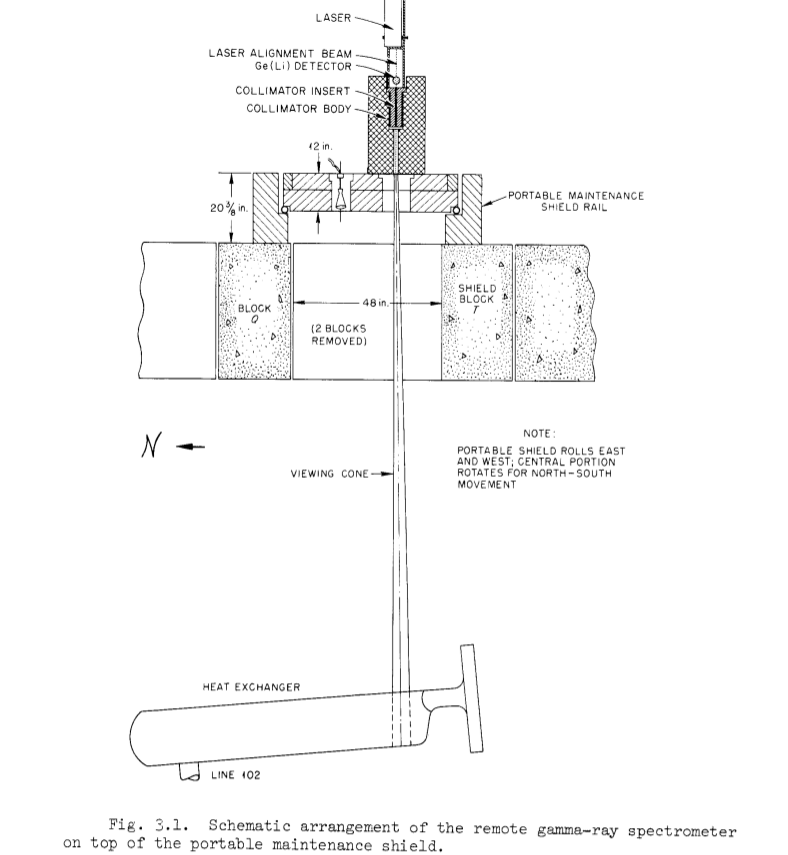
\includegraphics[width=0.8\textwidth]{Fig_3_1}
\caption{Schematic arrangement of the remote gamma-ray spectrometer on top of the portable maintenance shield.}
\label{Fig_3_1}
\end{figure}
图\ref{Fig_3_1}是这套设备的正面示意图,包括一个准直器、一个探测器和一个激光准直设备。图\ref{Fig_3_2}是设备的正视图实物图。在此图解中,这套设备被安置在可移动维护屏之上,但它也可以安置在钻有小洞的混泥土屏蔽罩上面。探测器是Ge(Li)晶体,连接适当的放大器到一个4096道的多道分析器。这样组合提供了高分辨率的能力。依赖$\gamma$射线强度,可以选择不同的嵌入式准直器。在可移动维护屏上使用这套设备时,通过激光准确定位测量的区域,透过可移动维护屏上的铅玻璃窗观察堆中的定位部位。这样可以通过移动可移动维护屏,达到精确定位。

\begin{figure}
%\graphicspath{{Figure/}}
\centering
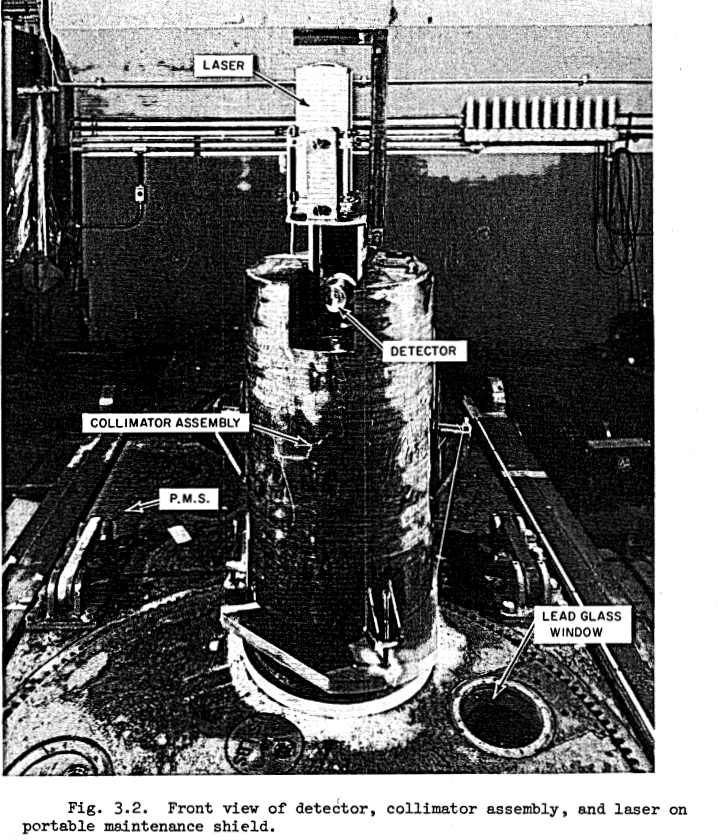
\includegraphics[width=0.8\textwidth]{Fig_3_2}
\caption{Front view of detector,collimator assembly, and laser on portable maintenance shield.}
\label{Fig_3_2}
\end{figure}

\section{探测器与前置放大器}
探测器是一个ORTEC公司制造的同轴锂漂移锗探测器,1333\ keV峰位的分辨率为1.78\ keV,直径36.65\ mm,长28.5\ mm,有效灵敏体积26.25\ $cm^3$,峰康比27/1。相对效率为4.3\%。配套ORTEC-440A或ORTEC-450放大器。

虽然到达探测器的准直射线强度挺强的,但是实际上和锗晶体发生作用的还是很少的。虽然设备并非在理想状态下用六个月的时间获得1400个能谱,但是整个系统的分辨率却没有变差。

\section{多道分析器}

使用Nuclear Data 2200系列4096道的多道分析器,所有谱保存到磁带。起先在操作分析器和磁盘时都会遇到一些问题,这些都是由于系统漏洞导致的。把多道分析器放置在一个高温且潮湿的环境中都会出现问题,使得系统在实验期间经常当机。

一旦把分析器和放大器放到控温、控湿的房间时,大部分问题都得到解决。用一条200ft的电缆连接前置放大器和主放大器,这么长的电缆对系统的系能影响可以忽略。由于当地供电系统不稳定(电压、频率不稳定),系统增益有时会有几道的漂移。高分辨率的探测器和4096道分析器满足当下的实验要求。反应堆运行时,一些堆组件(如热交换器、排气系统)中短寿命的裂变产物放射出的$\gamma$\ 射线杂音太多,导致能谱出现严重的重峰问题。这种情况下,在探测器和被测量区域之间加入适当的屏蔽来降低放射性强度,或者这样的谱不做处理。

\section{准直组件}

图\ref{Fig_3_3}展示了准直组件,其包括准直体、准直内插件,材质均为铅。准直体高32.5\ in,直径19\ in,中间有个圆孔用于嵌入准直内插件,准直内插件有三种不同孔径规格,分别位1/16、1/8、3/16\ in。

探测器和杜瓦瓶固定在准直体上的一个平台上,并可做微调处理。顶部的激光发出的光束通过准直内插件的准直孔,达到精确定位,在激光定位时,探测器和杜瓦瓶需要从准直组件上移出,也可以在不移动探测器和杜瓦瓶的情况下,通过一套复杂的光学系统达到精确定位。

\begin{figure}
%\graphicspath{{Figure/}}
\centering
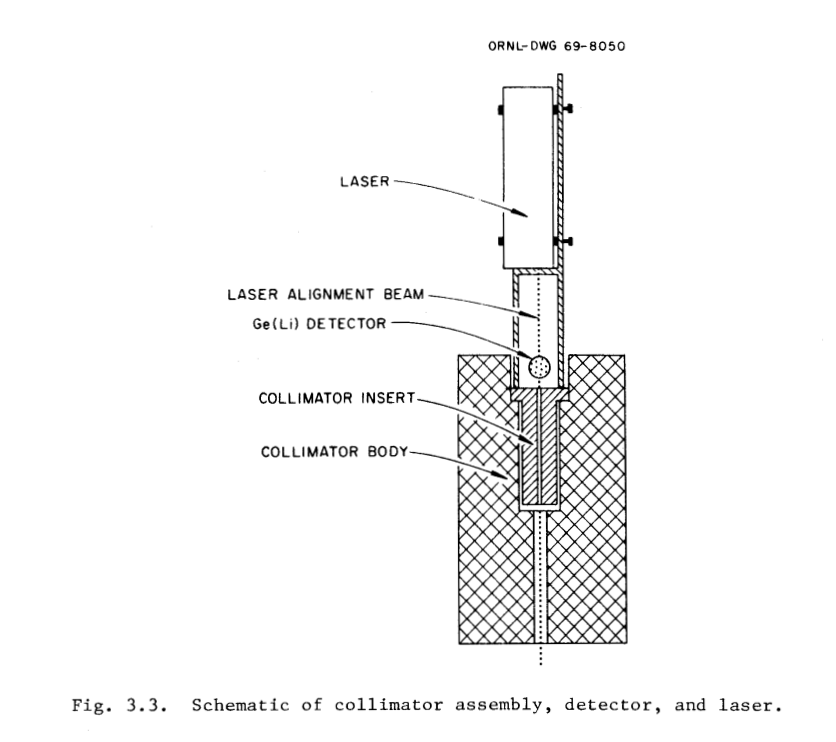
\includegraphics[width=0.8\textwidth]{Fig_3_3}
\caption{Schematic of collimator assembly, detector, and laser.}
\label{Fig_3_3}
\end{figure}

\section{实验设备安装}

停堆之后,需要花费几天的时间移出上层的屏蔽块和阻隔板,然后安装PMS和探测器装置。这种方式太长时间,所有决定在堆排气系统、主热交换器和排泄罐这三个需要观察的区域的屏蔽层打孔,这样就不用移动屏蔽层。在1969年停堆期间,打好这些孔。孔的校准通过人力移动上下屏蔽层,使其排成一条直线。把探测器和准直组件安置在屏蔽层上面,当停堆时,设备可立即工作,至少在这三个区域,就有机会研究较短寿命的核素。

使用PMS沿着热交换器轴线、燃料管路和排气管路观察裂变产物的放射性活度\footnote{R.\ Blumberg and E. C. Hise, MSRE Design and Operations Report.Part X. Maintenance Equipment and Procedure, ORNL-TM-910.}。图\ref{Fig_3_4}展示整个设备全貌。探测器和准直器安装在一个大的转盘上,因此能在PMS上自由转动。

\begin{figure}
%\graphicspath{{Figure/}}
\centering
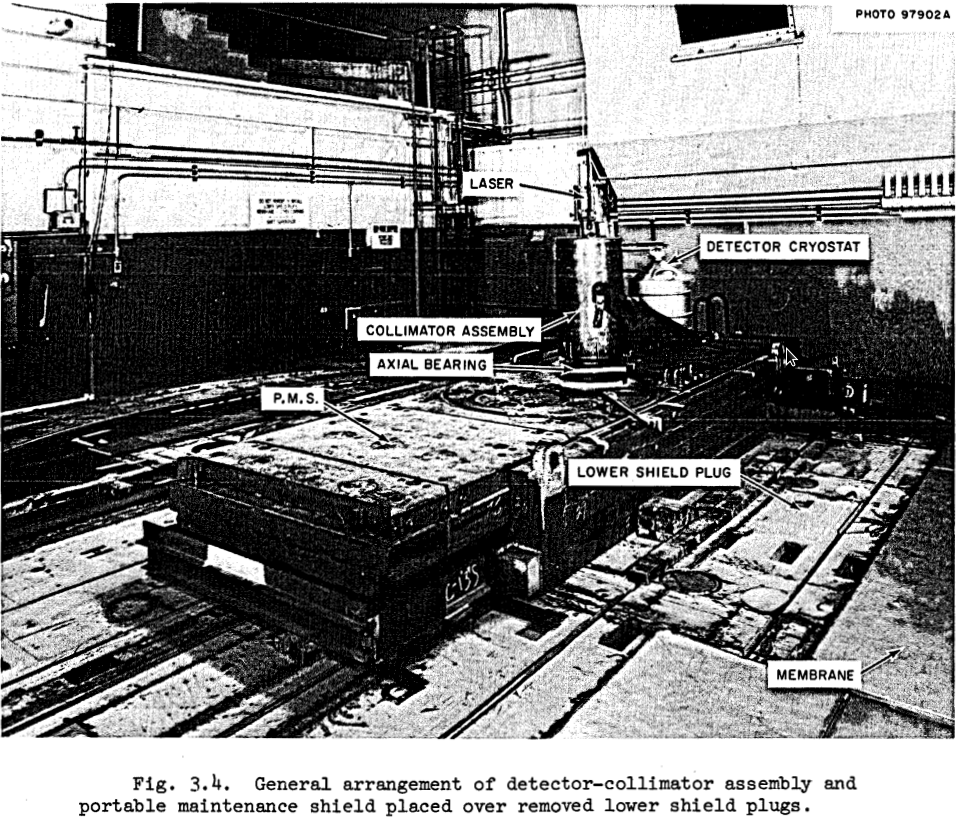
\includegraphics[width=0.8\textwidth]{Fig_3_4}
\caption{General arrangement of detector-collimator assembly and portable maintenance shield placed over removed lower shield plugs.}
\label{Fig_3_4}
\end{figure}

\section{定位设备}

精确定位获取$\gamma$\ 谱的组件位置是很重要的,本实验用一个低能激光和两个测量员的搬动实现这个目的。激光器固定在可调动的准直内插件上,激光束通过准直器中心孔洞,照射在将要测量$\gamma$能谱的位置上,出现一个红色斑点,这可以通过PMS上面的铅玻璃窗观看到。事先通过铅垂直线和水平仪调整,保证准直体水平,且激光束垂直。再配合测量员移动活动区,这样使定位系统精度达到1英寸以内。

\section{屏蔽}

如上面提到的各个堆组件,都有很强的放射性。当堆在运行期间,从覆盖在堆排气系统和热交换器之上的水泥屏蔽层的小孔测得的强度高于1000 R/hr。还有由快热中子引发的照射剂量。(除非采谱时,孔被堵塞,并用铅砖盖住。)

当堆满功率运行时,已经被证实不可能从热交换器上获得有用的$\gamma$谱图。熔盐回路中的很多裂变核素的光电峰叠加在一起,且偶然符合效应也产生很多无用的大叠加峰。计算程序就无法从这样的能谱分析出有用的信息。排气系统里所包含的核素种类比熔盐燃料少得多,但即使这样,反应堆满功率运行时在排气系统上测得的谱也是几乎没什么价值。为了得到排气系统上有用的谱图,需要使用一些屏蔽材料,如2英寸厚的浸有锂的煤油和1英寸厚的铜。(煤油中的锂用于吸收中子而不会发射出$\gamma$射线。)

当反应堆低功率运行或停堆时,就可以从热交换器和排气系统采谱分析。但仍然需要适当的屏蔽来保证探测器的输入计数率在合理的范围内,如3000-10000\ counts/sec。

现在面临的问题是需要许多好的屏蔽材料,如铅能大大降低低能$\gamma$\ 射线(能量低于几百keV)的强度,足够的铅屏蔽对更高能量的光子的强度也会有适当的减弱。因此,在这样的情况下,低能峰完全可以被屏蔽掉。由于低原子序数材料对低能$\gamma$射线没有好的屏蔽效果,铝或铜制的屏蔽可以克服这个缺点。从而,计数率可保持在一个理想的水平,同时允许较低能的$\gamma$射线测量。关于设备的刻度在第五章会有比较详细的描述。

通常,我们使用最少的屏蔽擦料和1/16\ in.规格的准直内插件,控制探测系统的死时间在低于25\%的水平下工作。

\section{刻度设置}

\begin{figure}
%\graphicspath{{Figure/}}
\centering
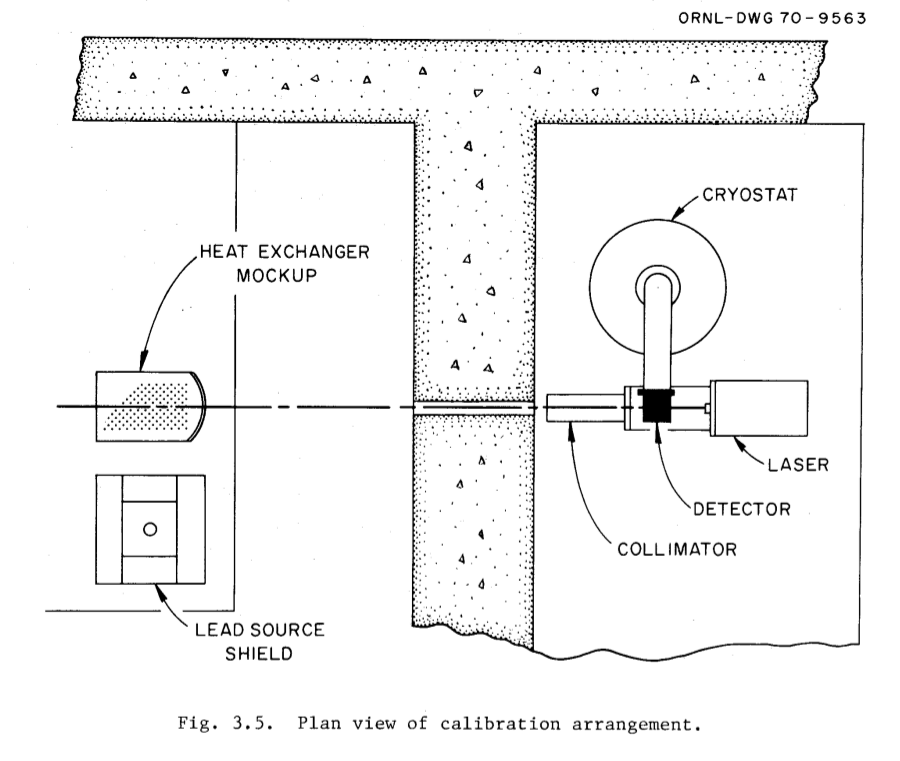
\includegraphics[width=0.8\textwidth]{Fig_3_5}
\caption{Plan view of calibration arrangement.}
\label{Fig_3_5}
\end{figure}

探测系统的效率是通过经验方式确定的,特别是热交换器的几何结构过于复杂,而无法通过理论计算来确保足够的精确。第五章将会给出复杂的刻度过程。附录D用简单的计算模型做了验证。

图3.5展示刻度实验的物理装置。探测器和一个准直器被安装在堆high-bay area中的一个地下单元(净化单元)。一个携带着放射管源的完整的主热交换器模型位于相邻的远程维护实践单元。固定在热交换器里面的放射源放出的射线穿过墙上的小孔和准直器,并和探测器相互作用。这堵墙足够厚,射线只能从准直器的小孔到达探测器。除了与模型直接接触的空间外,远程维护实践单元用普通的顶盖封闭;在此也用到PMS。通过PMS上的小孔,我们就可以借用简单的工具操作模型中的放射源和模拟热交换器的管子。

刻度实验中使用了活度24\ Ci(居里)$^{110m}$Ag 放射源。此放射源长6.3 in,直径0.5 in(真实的热交换器管道也是同样的直径),由橡树岭研究堆辐照活化得来。

使用设计的探测器测量此放射源放在热交换器模型的各个位置的放射性强度,这样就能得到热交换器各个点对探测器的响应情况。热交换器模型与探测器之间的距离与真实的热交换器和安装在PMS上的探测器的距离相当。

由于反应堆中的主排气线是一个直径1英寸的波纹管,对它刻度相对比较简单。通过对比放射源的管子,就可估计出它的刻度。

热交换器上的陶瓷部件以及为了如实观察热交换器和排气线而用到的屏蔽块也用相同的源做了刻度,估计其屏蔽能力,并与文献提供的数据计算做比较。为了达到目的,陶瓷发热器紧挨着放有管状放射源的热交换器的未屏蔽中心位置上。屏蔽块也是和远程维护实践间正面有孔的墙紧紧贴着。不同的屏蔽块的屏蔽能力和文献提供的计算结果符合。
%Description and performance of equipment
\chapter{谱分析}

\section{目的与操作概要}

分析$\gamma$能谱的目的是通过核素放出的特征$\gamma$\ 能量峰做到核素识别,如果考虑到探测系统的绝对计数效率,也能分析特定堆组件指定位置上的各种核素的含量。

在采谱时,4096道的多道器对应的每一道的计数都保存在多道器中的寄存器里面,停止采谱后,这些计数将保存到磁带上。其中,每一道计数都代表特定的能量间隔,且这个间隔大小是可调。一般实验条件下,一个能量间隔(也称为增益)控制在每道0.3-1.0 keV范围内。换句话说,获得的$\gamma$\ 能谱一般控制在1.2MeV($\sim$\ 0.3$\times$\ 4096)到4MeV(1.0$\times$\ 4096)之间。在一个谱中通过相邻几道的累积计数的增加来确定$\gamma$\ 射线峰(也称为光电峰或全能峰)的存在。实验证明光电峰的计数服从修正高斯曲线。峰的强度由峰高或更多的是高斯曲线峰面积表征。谱中的高斯峰顶点对应的道址即为$\gamma$\ 射线的能量。

$\gamma$\ 能谱分析一般有如下几个步骤:
\begin{enumerate}
\item 确定峰的道址;
\item 判断每个峰是否由统计涨落引起的或是真的光电峰,并且确定峰的起止点;
\item 通过相邻的道判断峰的本底;
\item 高斯曲线拟合峰型;
\item 计算峰面积,扣除对应的本底,即为$\gamma$\ 射线强度的测量值,同时通过高斯曲线的顶点精确定位峰的位置;
\item 查询核数据库,通过道址匹配核素对应的光电峰,确定峰对应的核素;
\item 由核素获得半衰期,$\gamma$\ 射线能量及对应的分支比,以及核素的母体和子体等信息;
\item 一旦核素被确定,计算峰面积即可求出此核素的活度。
\end{enumerate}

分析一个能谱要求探测器系统的效率(即对应的能量响应函数)必须包括需要观察的能量响应范围。同时,在分析过程中,$\gamma$\ 能量和峰道数要精确对应。典型的能谱如图\ref{Fig_4_1}\ 所示。

\begin{figure}
\centering
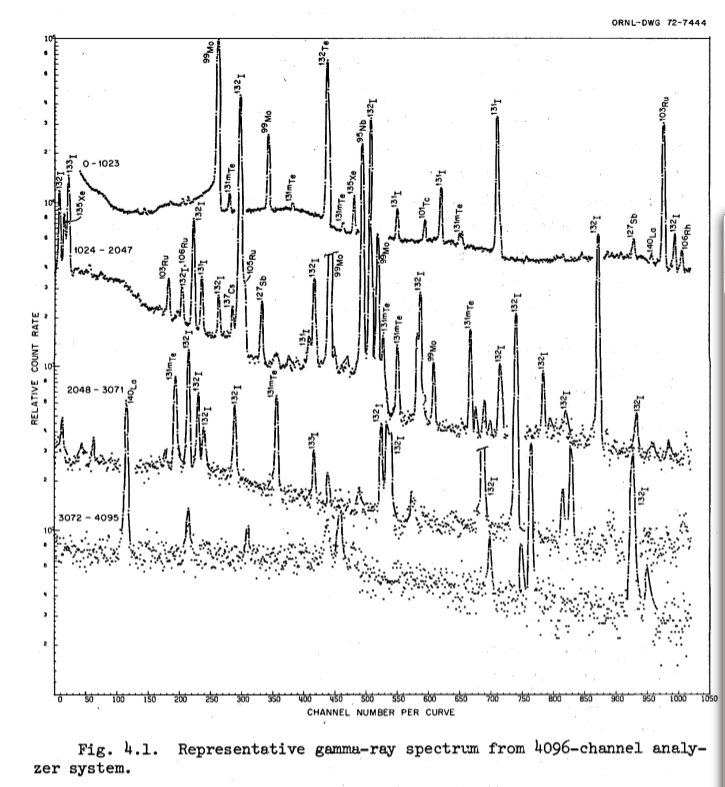
\includegraphics[width=0.8\textwidth]{Fig_4_1}
\caption{Representative gamma-ray spectrum from 4096-channel analyzer system.}
\label{Fig_4_1}
\end{figure}

\section{难点}
在停堆之后,很多短寿命的核素还没来衰变掉,此时采到的能谱里面的很多光电峰重叠在一起,这对增加谱的分析难度。例如,多重峰的起止点难以判断,其本底也无法扣除。重峰拟合主要靠多个高斯曲线左右移动叠加拟合。

如果有一个全面的包括射线能量及对应的分支比的核数据库,我们就能用射线的能量相对容易辨别核素。对于长寿命核素的的数据库比较全,但短寿命的缺少很多。

如上所示,全面地分析一个能谱是很困难,特别是手工解谱。因此,计算机自动化分析谱图将是不可或缺的,特别对于大量谱图而言尤为重要。

\section{同位素表}

本实验花费相当多的精力收集同位素数据。此数据库同时包含了长寿命和短寿命裂变产物的数据,这些数据来源于ORNL核数据项目组收集的最新文献。每个核素列出其$\gamma$\ 射线能量和对应的分支比,并按能量由小到大排列。同时,数据库也给出绝对$\gamma$\ 射线丰度、其前驱和衰变产物。这个表的使用对谱分析有很大的改善。本文给出的数据分析就是基于这张同位素表的。附录A给出了这个基本的同位素表。

以一个可能出错的问题为例,在分析$^{129m}$Te数据时,都会提到。首先这个核素有部分概率衰变到$^{129}$Te再到$^{129}$I,或直接由同核异能素衰变到$^{129}$I。这两种情况下,放出的$\gamma$\ 分支比都十分的小。

这就意味着在活度计算中乘一个大因子而放大了原始光电峰的统计误差。更令人不安的是整个$^{129m}$Te-$^{129}$Te衰变纲图还没有完全确定下来;文献资料提供了几种不同的衰变纲图。由于在$^{129m}$Te衰变中观察第二大光电峰(696.0keV)的同时也有其他核素放出此能量的射线,因此,我们不得不依赖459.6keV峰产生的结果。

基于最新可用的数据,我们评估出$^{129m}$Te衰变到$^{129}$Te再到$^{129}$I放射出459.6keV的分支比为4.9\%。不过随后提交的评估结果更为准确。$^{129}$Te衰变到$^{129}$I放射出459.6keV的分支比为7.7\%.

\section{计算机程序}

如前所述,计算机必须能正确处理本实验要分析的数据。现在最主要的问题是哪里能找到一个能分析存在多重峰的谱的程序。实验采得的谱的复杂程度为每个谱估计有150到230个峰。

ORNL数学部门开发了一个高效的$\gamma$能谱分析程序——GAMSPEC-3,但此程序不具备多重峰分析能力,且只能分析单峰不超过75个的能谱,也不能辨别核素类别。这些不足限制了很多谱的分析,尤其对存在短寿命核素的能谱。Gunnink\footnote{R. Gunnink et al., Identification and Determination of Gamma Emitters by Computer Analysis of Ge(Li) Spectra, LRL-UCID-15140.}等人开发了能满足本实验要求的多功能$\gamma$能谱分析程序——GAMANAl。此程序在劳伦斯放射性实验室(LRL)的CDC-6600计算机上用FORTRAN语言开发而来,又被阿贡实验室(ANL)的N.D.Dudey等人用FORTRAN-IV语言移植到IBM-360系列计算机上。通过ORNL数学部门的能力,此程序也在ORNL的计算机上正常运行。此程序花了LRL近五年的开发时间,ANL用两年时间移植到IBM-360计算机上,而ORNL用了4个月。

此程序实现峰定位(单峰、二重峰和三重峰)和通过峰位实现大量核素的辨别和计算。它能处理400个单峰,100个二重峰和100个三重峰。虽然此程序源于Gunnink,但本实验室做了一些改进,使它支持本实验室的核素数据库。例如源程序是读入一个多项式的系数作为整个探测系统的效率曲线,而本实验室改为用多对能量-效率曲线点就能自动得出相应的效率曲线。通常可支持60对能量-效率曲线点。为了减少纸张浪费,可用堆不同表格做不同的输出格式变化。

虽然此程序满足本实验大部分谱的分析工作,但依然存在一些问题:
\begin{enumerate}
\item{在一些特别的能量范围里,很多峰叠加在一起。此程序只能分析到3重峰,对于三重峰以上的就显得无能为力。}
\item{谱中短寿命核素太多,但核数据库又没有足够的信息,此种谱一般不做分析。}
\item{除非记录了所有核素的详细的衰变链,否则,当通过不同辨别测试方法,程序有时会由于找不到母体和子体而拒绝鉴别。唯一的方法是在能量库中分离母子体关系。例如,95衰变链中,$^{95}$Nb被分离出来而$^{95}$Zr依然在熔盐里。只要$^{95}$Zr作为母体,$^{95}$Nb在此程序中将无法鉴别。当然,这与程序的性能无关。}
\end{enumerate}
%Analysis of spectra
\chapter{刻度}

\section{概述}

刻度设备得出整个$\gamma$能谱测量系统的绝对效率曲线,同时考虑到准直组件和设备在反应堆单元中的物理布局。

在经验方法中,计数效率仅仅只是一个跟光电峰计数率和源强成比例关系,如下所示:
\begin{equation}
\label{eq:equ1}
CR\,=\,EF\,\bullet\,S
\end{equation}
其中,$CR$是计数率,$EF$是光电峰的探测效率,$S$是源强(单位源体积单位时间内发射的光子数)。应该指出,尽管$CR$由通过准直器的光子数决定,但是放射源强度仍然可由整个物体的某个或多个部分适当的表示出来。例如,在热交换器上(详见\ref{section:5_5}),准直器正对着充满放射性管的热交换器的圆锥体部分放射强度与期望的计数率符合。然而,源的强度等于单位时间单位面积的单管放出的光子数。因此,计数效率可表示为:
\begin{equation}
\label{eq:equ1}
EF(\frac{c}{\gamma/cm^{2}})=\frac{CR(counts/min)}{S(\frac{\gamma}{cm^{2}-min})}
\end{equation}
其中,$\gamma$表示发射的光子数,$c$表示被探测到的特定能量的光子数。热交换器上测得的计数率除以效率等于热交换器中放射管源每平方厘米光子发射率。在堆主排气线上,源强可用每分钟每英寸长度所发出的光子数$\gamma/in.-min$。探测系统的效率是关于$\gamma$射线能量的函数。通常,有两种方法确定能量和效率的关系。其一,先用几组不同的已知放射源测量探测器的简单几何模型下的效率曲线,再扣除准直器、距离、屏蔽、以及被观察的实际组件几何形状的影响,即可确定实际的效率曲线。其二,在实际的物理装置上用经验方法确定探测系统的效率。第二种方法相对比较简单且更可靠。然而,我们也使用更基本的近似去检查计算的可靠性。

\section{刻度源}

为了尽可能地模拟实际情况,实验选择直径0.5英寸银质管源,与主热交换器管道的直径相等。

由于$^{110m}$Ag在446.8——1562.2\ keV的能量范围内有多条$\gamma$射线,可便于效率曲线的计算。此外,用ORR的水力传送辐照装置制作这种放射源的代价相对便宜。由于银管对ORR堆的反应性有很大的影响,所以一般只有低2.3英寸长的管子才能用此装置进行辐照。因此,本实验分三次辐照此长度的银管。辐照样品前,先用注量监测片(Co-Al片)测量辐照位置的注量率和总注量。辐照之后在热室中处理样品,把这三个管源用不锈钢薄片包裹衔接起来(如图\ref{Fig_5_1})。附件B对源强和源各个位置活度变化率的计算做详细介绍。

\begin{figure}
\centering
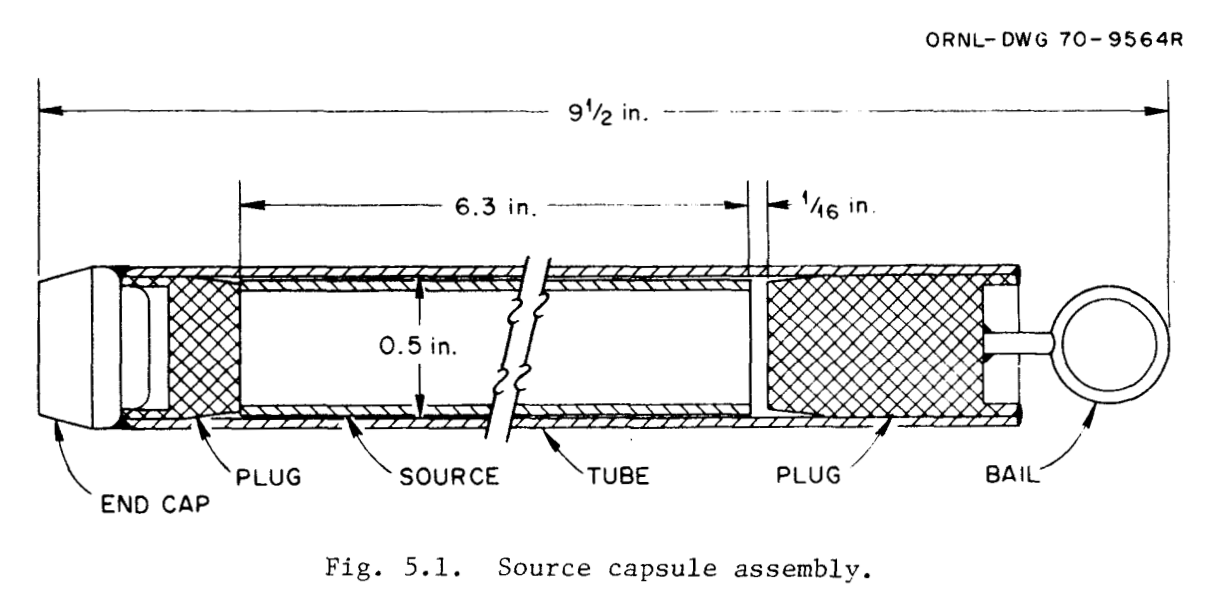
\includegraphics[width=0.8\textwidth]{Fig_5_1}
\caption{Source capsule assembly.}
\label{Fig_5_1}
\end{figure}

\section{狭缝实验——放射源强度}

由于ORR堆中的中子通量分布各异,导致管源在长度上的活化率不一。为了正确刻度探测系统,就必须知道管源活化率的情况。起先,计划通过测量管源上各点$^{110m}$Ag的活度和通量监测片上获得的活化率来推算$^{110m}$Ag的放射性水平(附录B中的表B.2和B.4)。然而,这样处理有很多不确定性。一个更好的处理方法是使用Ge(Li)探测器和准直器区扫描管源。在MSRE的远程维护间(RMPC)中用铅砖堆出一个高两英尺的狭缝,缝宽1/8英寸;一个管源能顺利穿过的玻璃管紧挨着垂直固定在狭缝上。探测器放置在隔壁的去污间,并紧挨在正对狭缝的小孔上。当放射源置于玻璃管之中时,银管1/8英寸处的$\gamma$射线能穿过狭缝、墙体的小洞和准直器,并打到探测器。把源降到狭缝下面,然后开始扫描探测,逐渐提高放射源,直到探测器示意到源的顶部在缝的前面。

在扫描时,以1/8英寸的步长向上移动源并获取相应的$\gamma$能谱,直到整个源都通过狭缝。解谱并画出源位置与光电峰净面积的曲线关系即可得到源的放射性强度的分布轮廓(见\ref{Fig_5_2})。由这些结果可以计算沿管源轴向方向上任何一点的绝对活度(见附录B)。

由于管状银源的活度分布不是完全的均匀,准直器要指向管源有意义的部位,所以计算源强的平均值对于系统来说是十分必要的。源强平均值$\overline{S}$可表示为:
\begin{equation}
\label{eq:equ3}
\overline{S}=\frac{\int_{0}^{L} S(x) R(x) dx}{\int_{0}^{L} R(x) dx}
\end{equation}
其中,$L$为管的长度,$S(x)$为$x$点的源强,$R(x)$为加权函数相当于轴向计数效率(点源的灵敏度响应函数即为源到准直器轴向的距离函数)。在狭缝实验中发现源强$S(x)$和计数率$CR(x)$呈线性相关,因此,式\ref{eq:equ3}可写为:
\begin{equation}
\label{eq:equ4}
\overline{S}=\frac{k \int_{0}^{L} CR(x) R(x) dx}{\int_{0}^{L} R(x) dx}
\end{equation}
其中,$K$是$S(x)$相对于$CR(x)$的比例常数。注意在狭缝实验设置中$K$为源的计数效率的倒数,其单位为(y/in.)/c.。由此可得:
\begin{equation}
\label{eq:equ5}
\overline{CR}=\frac{\overline{S}}{K}=\frac{\int_{0}^{L} CR(x) R(x) dx}{\int_{0}^{L} R(x) dx}
\end{equation}
其中,$\overline{CR}$为整个源管对应的某一$\gamma$射线的平均计数率。

为了确定权重函数$R(x)$,假设准直探测器组件具有旋转对称性;也就是 说,只能从准直轴方向做径向移动。(这个假设要求准直器的小洞要非常直,这看起来是有道理的,至少对1/8英寸的准直器来说。)

在热交换器模型的刻度工作(看\ref{section:5_5})中,可以测量探测器对源从准直器轴的左边到右边的计数率的分布贡献。图\ref{Fig_5_3}为探测器对银管源的轴向各点的归一化灵敏度曲线图。此图由如下数据构成:在热交换器模型的每列管的放射性管源位置上测出$^{110m}Ag$的三个不同光电峰的净计数率(平行于准直轴,如\ref{Fig_3_5})。概括整列的读数的原因是为了获得一个更统一的放射源分布,以及更好的计数统计。通过这个模型的计数率分布,归一三个光电峰到某个统一的值,且纠正准直器的轻微错位。图\ref{Fig_5_3}显示三条归一化曲线的平均值,这个平均值的偏差很小。这幅图也代表了权重函数$R(x)$。乘以管的计数率所得的结果就是探测系统中所看到的源的总有效活性,该计数率通过狭缝实验\ref{Fig_5_2}得到,符合探测器中所看到的归一分布规律。管源选择的三个能量峰的平均计数率等于图\ref{Fig_5_4}中对应的三个面积分别除以图\ref{Fig_5_3}中归一曲线下的面积。我们得到的三个源的加权后的计数率:

%\begin{table}
%\centering
\begin{tabular}[c]{ccc}
\hline
Energy (keV)  &  Count rate (counts/min) \\
\hline
657.7  &  27,500  \\
884.7  &  24,300  \\
937.5  &  13,600  \\
\hline
\end{tabular}
%\end{table}

知道了在不屏蔽条件下这三个能量峰的平均计数率,只需要计算$k$\ 就能确定源的平均强度。

\begin{equation}
\label{eq:equ6}
k_i(x)=\frac{S(x))}{CR(x)}
\end{equation}
$S(x)$\ 与$CR(x)$\ 分别为源在点$x$处的强度和对应的计数率,这些值在狭缝实验中测到。下标i表示第i条$\gamma$\ 射线。既然知道源中两个点的强度(看\ref{Fig_5_2}和附件B),既可以使用狭缝实验得到的结果来计算三条$\gamma$\ 射线在这两点上的$k$。如下所示:

\begin{table}
\centering
\caption{Count rates measured at two positions along the silver source for 	three different photopeaks}
\begin{tabular}[c]{cccccc}
%\caption{Count rates measured at two positions along the silver source for 	three different photopeaks}
\hline
%Photon  &  Count rate from & & Count rate from & \\
%energy &	slit experiment &   $k$(x10$^4$) &  slit experimen & $k$(x10$^4$) 
%&   $\overline{k}$ (x10$^4$) \\
%	&for 3.861 Ci/in.   &    &  for 4.196Ci/in. \\

%\tabincell{c}{Photon \\ energy} & \tabincell{c}{Count rate from \\ slit 
%	experiment \\ for 3.861 Ci/in.  } & $k$(x10$^4$) & \tabincell{c}{Count rate from \\ slit 
%	experiment \\ for 3.861 Ci/in.} &  $k$(x10$^4$) & $ \overline{k}$ (x10$^4$)  \\

\multirow{3}{2cm}{Photon energy} & \multirow{3}{3cm}{Count rate from  slit 	experiment for 3.861 Ci/in.} &  \multirow{3}{2cm}{$k$(x10$^4$)}& \multirow{3}{3cm}{Count rate from  slit experiment  for 3.861 Ci/in.} & \multirow{3}{2cm}{$k$(x10$^4$)}&  \multirow{3}{2cm}{$\overline{k}$ (x10$^4	$)} \\
%& &$k$(x10$^4$) &  & $k$(x10$^4$) &  $ \overline{k}$ (x10$^4$) \\
\\
\\
(keV)& (counts/min) & $\frac{Ci/in. }{counts/min}$  & (counts/min)  & 
$\frac{Ci/in.}{counts/min}$ &   \\
\hline
657.7  &  25,900  &1.491  &28,300  &1.481  &1.486  \\
884.7  &  23,100  &1.675  &25,100  &1.671  &1.673  \\
937.5  &  12,700  &3.044  &14,700  &2.861  &2.953  \\
\hline
\end{tabular}
\end{table}

列出管源上标定位置点上对应的$\gamma$\ 射线的计数率和$k$\ 。此外,也列出管上两点的$k$\ 平均值。通过这些$k$\ 的平均值乘以上面列出的三条$\gamma$\ 射线对应的平均计数率,即可算出源的三个平均强度。计算结果如下:

%\begin{table}
%\centering
\begin{tabular}[c]{ccc}
\hline
Energy (keV)  &  Source strength (Ci/in.) \\
\hline
657.7  &  4.09  \\
884.7  &  4.07  \\
937.5  &  4.00  \\
\hline
\end{tabular}
%\end{table}

由此可算得管源的平均强度为4.05\ Ci/in. 
。

由于使用平面源(源置于热交换器模型内各个位置)去估计线源的权重因子,因此,此类源评估方法过于理想,具有一定的误差。然而,归一化权重曲线\ref{Fig_5_3}两边急剧上升,中间源活度变化平稳,因此,此方法应该是可行的。考虑到评估源的放射性强度和权重因子的误差,估计计算源强度的误差在$\pm5\%$。

\begin{figure}
\centering
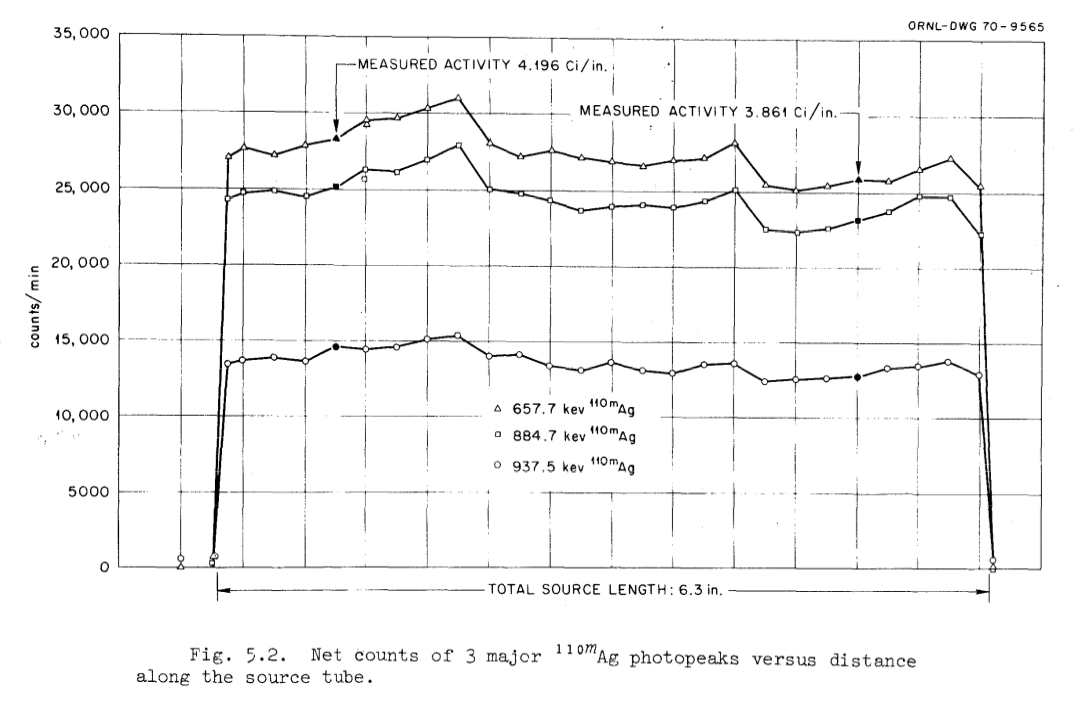
\includegraphics[width=0.8\textwidth]{Fig_5_2}
\caption{Net counts of 3 major $^{110m}$Ag photopeaks versus distance along the source tube.}
\label{Fig_5_2}
\end{figure}

\begin{figure}
\centering
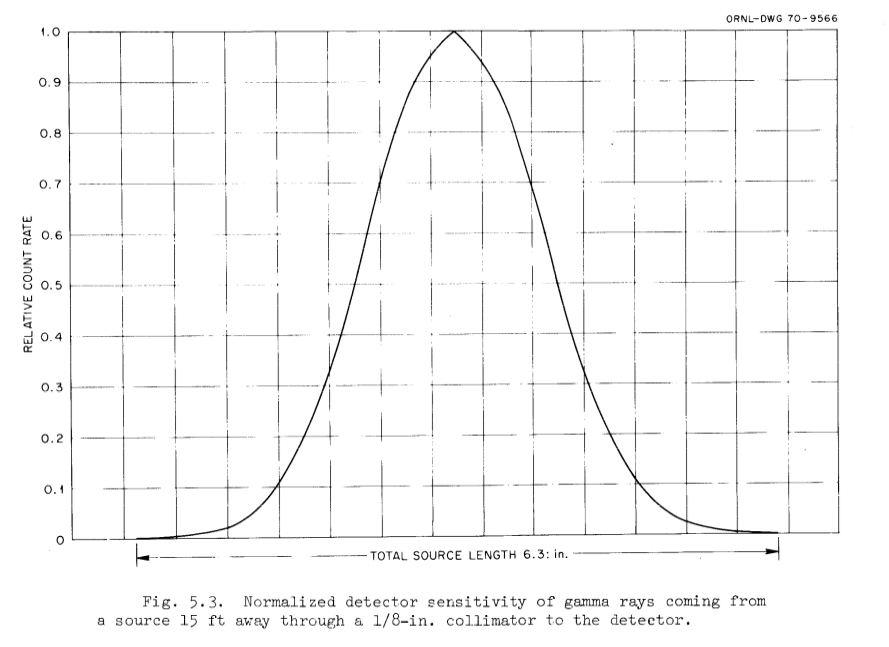
\includegraphics[width=0.8\textwidth]{Fig_5_3}
\caption{Normalized detector sensitivity of gamma rays coming from a source 15\ ft away through a 1/8-in. collimator to the detector.}
\label{Fig_5_3}
\end{figure}


\begin{figure}
\centering
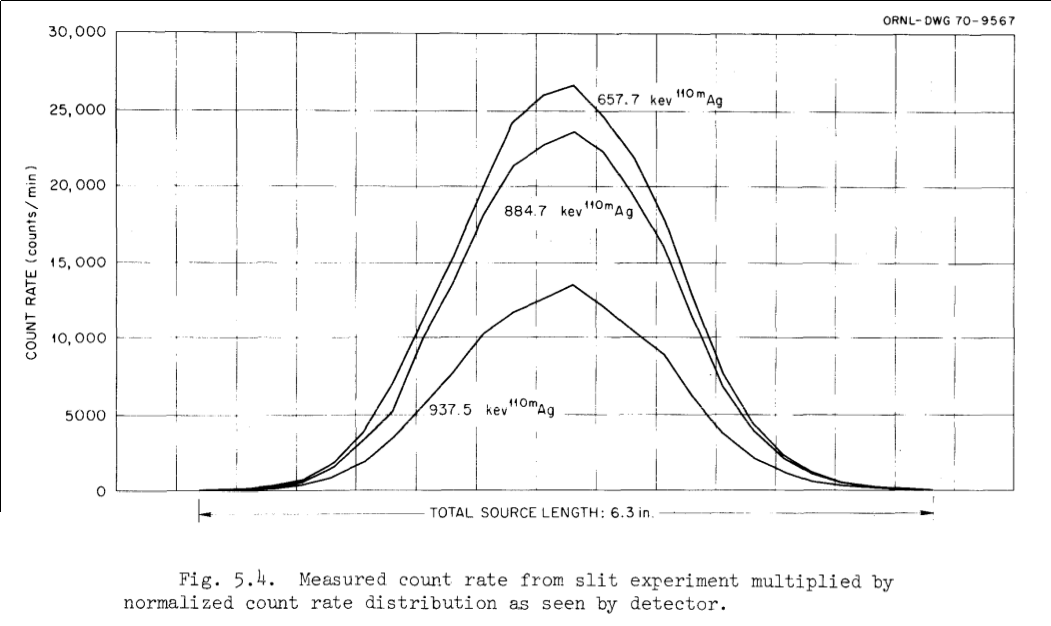
\includegraphics[width=0.8\textwidth]{Fig_5_4}
\caption{Measured count rate from slit experiment multiplied by normalized count rate distribution as seen by detector.}
\label{Fig_5_4}
\end{figure}

\section{单放射源实验}

单源实验是为了刻度用于测量反应堆中主排气线的$\gamma$\ 射线的探测系统的效率。假设探测器对$^{110m}$Ag管源和直径1英寸的折叠主排气线有相同的计数效率。管源安装在未屏蔽的热交换器模型的中心位置, 准直器由激光校准。微调准直器使得设备获得最大的计数率。管源到探测器的距离大约等于PMS上的探测装置到堆单元中的主排气线的距离。使用$1/8$英寸内径的准直内插件。

依据实验获得的数据和不同$\gamma$\ 射线($^{110m}$Ag的15个光电峰)的绝对分支比,我们能算出探测系统在这些能量点上探测效率。用$^{110m}$Ag的446.8keV到1562.2keV的$\gamma$\ 射线估计出探测器的绝对效率曲线。由于很多裂变产物的光电峰不在此能量范围内,所以需要扩展效率曲线去突破这些限制。决定使用从排气线上获得的裂变产物谱来扩展效率曲线的能量范围。例如,使用$^{99}$Mo,$^{131}$I,$^{132}$I和$^{140}$La的140到2522keV能量点作出相对效率曲线。再匹配$^{110m}$Ag的绝对效率曲线,即可获得一条宽能量范围的绝对效率曲线。图\ref{Fig_5_5}为堆内排气线采用的效率曲线。

同时使用光电峰超出能量范围的$^{226}$Ra源去检查上面的方法。此源得到的相对效率曲线的形状基本上与绝对效率曲线的一样。它们的差异可能是由于实际发射光子对屏蔽的不同表现引起的,在低能端尤其明显。


\section{热交换器刻度}\label{section:5_5}

热交换器刻度是通过热交换器模型的整体尺寸进行刻度。8.5英寸长的模型管子的外直径和壁厚与实际的热交换器管子一样。在模型中,这些管被垂直固定在两个相距约6英寸水平板上,且以边长为0.775英寸的正三角形排列。借助简单的工具,可以容易在PMS上的操作孔中操控这些管子。这个模型包含20行管子(与探测器准直器轴向垂直)。由于呈正三角形排列,每行有八或九个管子。为了模拟热交换器的壳层,在模型前面适当位置放置一个厚0.5英寸的不锈钢曲面。

在这个模型中任选某个管位插入一个放射性管源,其他所有管位用仿造管代替,然后进行采谱。这样操作进行两遍,一次用4400A放大器,一次用450型号的;使用1/8英寸准直器。

通过相加模型中的所有源位置的对应谱的$^{110m}$Ag各个光电峰的计数率,获得的计数率代表主换热器在每根管子每英寸4.06\ Ci\ $^{110m}$Ag的活度,但这也包括换热器其他所有管子的整体屏蔽作用。考虑到实验数据和$^{110m}$Ag各个$\gamma$射线的分支比,我们可以建立446.8~1562.2keV能量段适用用于换热的绝对效率曲线器。同时,使用两个不同放大器获得的数据之间存在很小的差异;我们使用这两条曲线的平均值作为标准。

来源于主换热器的裂变产物数据也扩展了效率曲线的能量相应范围;使用来自$^{99}$Mo、$^{131}$I、$^{132}$I的光电峰,以及少量的$^{140}$La(在空换热器中存在少量的$^{140}$La)。发热器元素的屏蔽效应被单独测量和计算。最终的标准效率曲线如图\ref{Fig_5_6},其中包括了换热器的壳层和发热器盒子的影响。与排气线相反,这条曲线在低能端向下弯曲。这种现象是由于换热器的内部屏蔽作用,因此,随着光子能量的降低光子的衰减系数剧烈下降。在初次使用计算机程序时,这种现象可能出现问题。

上述的刻度操作未能考虑沉积在换热器壳层内表面的裂变产物的影响。然而,和沉积在管道上的数量相比,这个的影响更小。另一个限制是只有当所有裂变产物均匀沉积在管上时,这个刻度方案才是可行。虽然这未必是真实的,但也没有证据来支持其他近似。

为了检验这个经验效率刻度,我们从基本原理上分别计算了线源对应的银管和堆排气线、体源(截锥体)对应的准直器对准的换热器弧面的计数效率。详情见附录D。我们确信,实验和计算值符合一致增强了测量的可靠性。

\begin{figure}
\centering
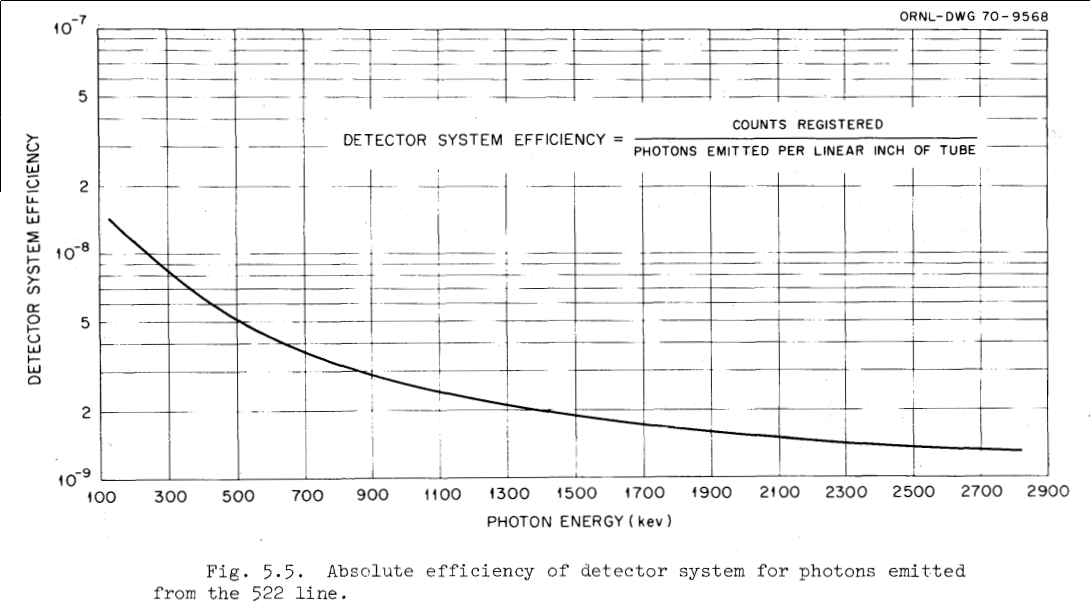
\includegraphics[width=0.8\textwidth]{Fig_5_5}
\caption{Absolute efficiency of detector system for photons emitted from the 522 line.}
\label{Fig_5_5}
\end{figure}

\begin{figure}
\centering
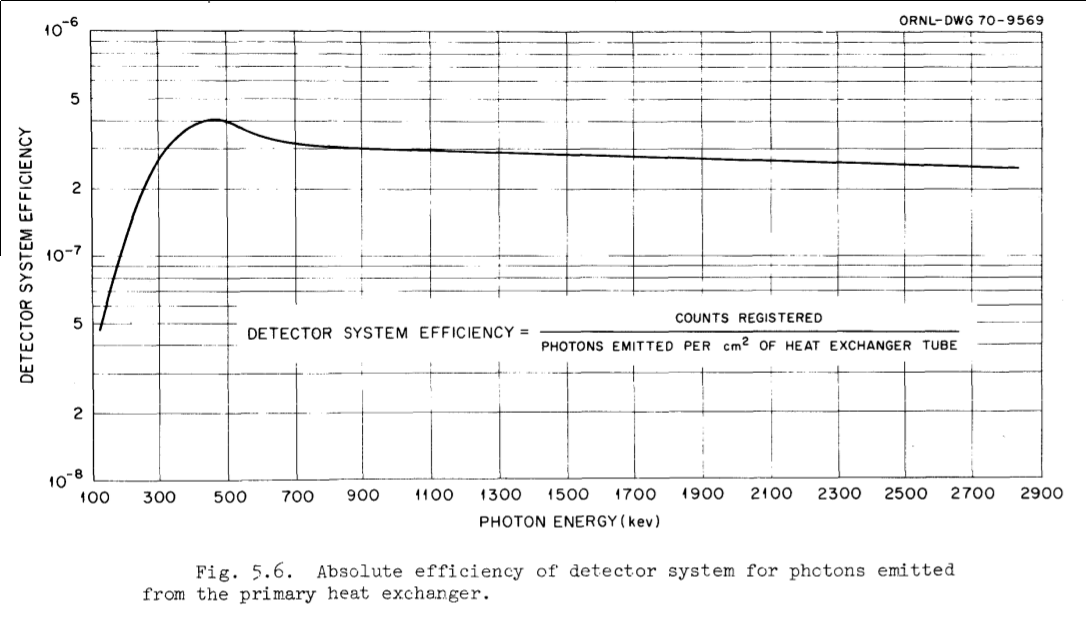
\includegraphics[width=0.8\textwidth]{Fig_5_6}
\caption{Absolute efficiency of detector system for photons emitted from the primary heat exchanger.}
\label{Fig_5_6}
\end{figure}

\section{屏蔽材料刻度}
整个实验过程中,保持探测系统的总计数率在3000-10000\ cps之间。由于源强随时间和位置的变化而变化,所有通过在探测系统和源之间插入不同的屏蔽材料来改变探测效率。在大多数情况下,用厚1/2英寸、直径7英寸的圆盘放置在PMS和准直组件之间。在激光定位时,这种圆盘容易移出。这种圆盘的材质包括铝、铜以及浸有锂的煤油。对于一些极端高放射强度水平,就得在准直体和探测器之间使用厚1/4英寸的铅盘。铅屏蔽除了有较大的衰减系数,特别对低能射线,这种材料也会和射线作用产生X射线而干扰探测。在评估不同屏蔽材料的影响时,不仅仅依赖于公布的衰减系数,也要对屏蔽圆盘做校准。使用了未屏蔽的银源和$^{226}$Ra\ 源做此事。文献提供的pb、Cu、Al、Cd和钢的衰减系数与实验值吻合;对于浸锂石蜡和换热器的陶瓷加热元件的值不得不依赖实验来获得。为所有不同的屏蔽材料绘制所谓的“屏蔽曲线”;所绘制的曲线是屏蔽系数(通常是衰减系数的倒数)在140-2500\ keV能量段的函数。

绝对效率曲线包含了实验用到的各种屏蔽材料的影响。非屏蔽效率值逐点除以屏蔽因子即可得到适当的屏蔽结果。当有多种屏蔽圆盘用到时,联合屏蔽系数计算如下:
\begin{equation}
%\label{eq:equ3}
EF_S(E)=\frac{EF_u(E)}{\prod [A_i(E)]^{N_i}}
\end{equation}
其中,$EF_S(E)$为有屏蔽体时能量E对应的效率;$EF_u(E)$为无屏蔽体时能量E对应的效率;$A_i(E)$为第i种屏蔽组件的屏蔽因子;$N_i$为第i个组件的个数。

总之,在堆主排气线上用了12种不同的屏蔽组件,而换热器的有8种,如表\ref{table_5_2}和\ref{table_5_3}所示。包含了材料屏蔽影响的效率曲线值输入到计算机分析程序中,用于评估出现的核素的绝对含量。附录C给出了不同的效率曲线。

在停堆或排料时,主要使用一些简单的铝或铜材质屏蔽体。而在不同堆功率下时,由于中子辐照和高能$\gamma$射线的存在,我们不得不用上更多屏蔽体。停堆后在不同时段用不同的屏蔽配置采集同一个位置大量的$\gamma$谱图,分析大量的沉积核素得到同样的结论;这使我们对当前使用的绝对效率曲线有一定的信心。

\begin{table}
\centering
\label{table_5_2}
\onelinecaptionsfalse
\caption{Shielding configurations employed during \protect\\
	surveys of reactor off-gas line}
\begin{tabular}[c]{ccl}
\hline
\multirow{3}{2cm}{Shielding case} & \multirow{3}{2cm}{Collimator insert 
	diameter(in.)} &  \multirow{3}{4cm}{Shielding material}\\
		\\
		\\
\hline
1  &  1/16  & 1/8\ in. steel  \\
2  &  1/8  & 1/8\ in. steel,1\ in.  Cu  \\
3  &  1/16  & 1/8\ in. steel,1\ in.  Cu,2\ in.  paraffin(Li),1/8\ in.  Cd  \\
4  &  1/8  & 1\ in. Al  \\
5  &  1/8  & None  \\
6  &  1/16  & None  \\
7  &  1/8  & 1/8\ in. Cd  \\
8  &  1/8  & 1/8\ in. Cd,1/8\ in.  steel  \\
9  &  1/16  & 1/8\ in.  Cd,1/8\ in. steel  \\
10  &  1/16  & 1/8\ in. Cd,1/8\ in.  steel,2\ in.  paraffin(Li),1/2\ in.  Pb  \\
11  &  1/16  & 1/8\ in. Cd,1/8\ in.  steel,2\ in.  paraffin(Li),1/4\ in.  Pb  \\
12  &  1/16  & 1/8\ in. Cd,1/8\ in.  steel,2\ in.  paraffin(Li) \\
\hline
\end{tabular}
\end{table}

\begin{table}
\centering
\onelinecaptionsfalse
\caption{Shielding configurations employed during \protect \\ surveys of primary heat exchanger}
\label{table_5_3}
\begin{tabular}[c]{ccl}
\hline
\multirow{3}{2cm}{Shielding case} & \multirow{3}{2cm}{Collimator insert 
	diameter(in.)} &  \multirow{3}{4cm}{Shielding material}\\
		\\
		\\
\hline
1  &  1/8  & None  \\
2  &  1/8  & 1\ in. Al \\
3  &  1/8  & 1/2\ in. Al,1/2\ in.  Cu  \\
4  &  1/8  & 1/2\ in. Al,1/2\ Cu  \\
5  &  1/8  & None  \\
6  &  1/16  & 1/8\ in. steel  \\
7  &  1/8  & 1/8\ in. Cd  \\
8  &  1/8  & 1/8\ in. Cd,1/8\ in.  steel  
\\
\hline
\end{tabular}
\end{table}

为评估1/16英寸准直插入件相对于1/8英寸的影响而做了大量的实验。在刻度实验过程中,发现使用1/16英寸插入件所降低的计数率明显高于4倍;同时单独测量时也考虑了散射影响。由于准直轴和银管中心存在轻微的错位,引起更大的误差。因此,在其他实验中,用一个轻薄活动片对准直件和探测器的末端进行微调节。相对于1/8英寸内插件,1/16英寸的屏蔽系数为9.0。这个测试做了多次验证,实验值误差在$\pm10$\%。显然,1/16英寸准直器还是不够直。


\section{MSRE中裂变气体刻度}

由于刻度所使用的刻度源来源于沉积在换热器冷却管里的放射源,计算机程序获得的结果都以这样的方式表示,包括气体。虽然气体的“等效表面沉积”模型在表示其浓度上是有效模型,但是在某些方面上根据换热器的截面体积去表示它们的浓度更有用。计算了有用体积与表面积的平均比率为0.55$cm^3/cm^2$。因此,气体的结果可以用每分钟每立方厘米的衰变数除以每分钟每平方厘米的衰变数再除以0.55。


%Calibration
\chapter{测量}
在1969年七月到十二月期间,在堆不同位置(如图\ref{table_6_1})总共采集了1400多个$\gamma$\ 谱图。做这些测量的目的如下:

A组:自1969年6月1号起,堆停止运行且排出熔盐。此时测量是为了检验设备,也为了研究长寿命裂变产物。

B组:在堆从低功率到满功率运行的几个级别上。改变堆状态,如燃料泵速,燃料泵中氦净化气比例率,变为氩净化,裂变气体的浓度,如$^{135}$Xe。这些谱图在一个塞有减弱片的小孔是获得的,并由另一篇报告报道。

C组:由$^{110m}$Ag、$^{226}$Ra源做的刻度谱图。第5章做了详细介绍。

D组:在加入铍的前后,在堆排气线上采集少数的谱图,分析加入铍是否引起裂变气体浓度的变化。结果在文献15报道。

E组:在燃料泵下游几百英尺的堆排气线上记录一些谱图。目的是研究裂变气体浓度。

F组:停堆和排料需要几天时间,架设可移动式维护屏蔽件也需要时日,这段时间内使用屏蔽插件可以获得一些谱图数据,堆在1969年11月2号开始排料。在这段时间有大量的裂变产物排出,通过谱测量可以研究沉积在系统里的裂变产物。

G组:停堆后,在可移动式维护屏蔽间上架设探测系统,这是本次实验最重要的数据来源。

H组:有一些谱在对着换热器的小孔是获得的。这些谱分别在堆满功率运行、停堆、排料及其之后采集的。

I组:停堆之后,采集堆内气体样品,记录其$\gamma$能谱,用于停堆之后分析是否管道泄漏。

J组:排料之后,记录熔盐冷却剂的放射性探测器放置在散热器管道前。目的是寻找任何沉积在散热管上的放射性的腐蚀物质。

k组:测量主冷却剂管道上两个点的$\gamma$能谱,根据熔盐冷却剂中$^{20}$F、$^{16}$N的衰变研究冷却剂的流速;$^{20}$F、$^{16}$N由换热器中燃料盐的缓发中子引起的。

L组:采集来自燃料泵和样品采集器采集的燃料盐、石墨样品。

M组:各种样品谱图,如来自润滑油系统,空气过滤器,排气线是的渗出物。

各种能谱的分析结果在第六章报道。


\begin{table}
\centering
\onelinecaptionsfalse
\caption{Gamma-ray spectra recorded\protect \\July to December 1969}
\label{table_6_1}
\begin{tabular}[c]{clcr}
\hline
\multirow{3}{1cm}{Group } & \multirow{3}{2cm}{Place} &  
\multirow{3}{2cm}{Time}&  \multirow{3}{1cm}{Number of spectra}\\
		\\
		\\
\hline
\\
A  &  MSRE heat exchanger  & July  & 114  \\
   &  Main reactor off-gas line(522 jumper line) &   & 20 \\
   &  Main fuel line (line 102) &  & 5  \\
B  &  Through shield plug hole over off-gas line  & Aug.-Sept.  & 235  \\
   &  Through shield plug hole over heat exchanger &  & 15  \\
C  &  Calibrations (chap. 5)  & Oct.  & 425  \\
D  &  Though shield plug hole over off-gas line (during Be addition)  & Oct.  & 9  \\
E  &  Main off-gas line in vent house   & Oct.  &6  \\
F  &  Through shield plug hole over heat exchanger   & Nov.  & 18  \\
   &   Through shield plug hole over off-gas line  & & 24  \\
   &  Through shield plug hole over drain tank  &  & 15  \\
 G &  MSRE heat exchanger   & Nov.  &241  \\
  &   Main reactor off-gas line (522line) & & 91  \\
  &   fuel pump bowl, fuel lines (line 101 and 102) &  &36  \\
 H &  Through shield plug over heat exchanger; final shutdown  & Dec.   & 43 \\
 I &  Gas samples, reactor cell  & Dec.  &9  \\
J  &  MSRE coolant salt radiator  & Dec.  &5  \\
K  &  Main coolant line  &Dec.   &14  \\
L  &  Samples of fuel salt and graphite  &Dec.   &45  \\
M  &  Miscellaneous:lube oil system, 523line roughing filters  &July-Dec.   &10  \\
\\
\hline
\end{tabular}
\end{table}


%Measurements
\chapter{结果}

本章根据上一章列出的测量谱排序,详细描述MSRE中裂变产物的分布情况。由于谱图数量多,其结果主要以图表的形式呈现,对于一些明显错误的数据,将直接舍弃。

\section{A组谱}

A组谱是在停堆期间时记录的,采谱点为换热器,主排气线,熔盐回路。大多数谱是在停堆6周后获得(1969.6.1),意味着只有一些长寿命的核素存在,谱图也相对简洁,无重峰现象。谱的采集时间约为200秒。有多条$\gamma$\ 射线的核素,只用比较显著的光电峰得出的活度的均值作为结果。

虽然$^{137}$Cs和$^{140}$Ba—La多次在换热器中被检测到,但它们的活度太低,推测是在停堆排空后,系统中的Xe衰变后沉积的结果。$^{95}$Zr未被检测到。本段列出的结果由指数倒推到停堆时刻计算得出的,倒推的结论可以与不同时刻采谱得出的结果相比较,然而倒推值由于母体衰变的影响而偏高。如$^{131}$I倒推值由于$^{131m}$Te的衰变而偏大。

\subsection{换热器}

沿换热器的纵向采得65个谱,水平方向四个点上采集49个谱。由于换热器的屏蔽状态的变化,如换热管数目的变化,光子通过换热器时的强度衰减,无法对水平方向进行定量分析。而裂变产物在纵向上是对称分布的。在换热器连接盒(HTR plug)处采集的谱图由于涉及未知的屏蔽参数,而无法做定量分析。此处的结果远低于其他谱,这不是由于裂变产物的不同沉积引起的。

\underline{Ni-95 \ref{fig_7_1}} 沿换热管纵向的衰变率在$0.1\sim 0.3\times 10^{12}dis/min/cm^2$,在阻挡板附近,值为$0.25\sim 0.3\times 10^{12}dis/min/cm^2$,在阻挡板之间的值$0.1\sim 0.15\times 10^{12}dis/min/cm^2$位于壳上侧的阻挡板的活度明显增大,推测是由于靠近挡板和壳位置的流速较低引起的。由图似乎观察不出活度沿着换热器纵向存在规律性变化。

\underline{Ru-103} 沿着纵向的衰变率几乎与$^{95}$Nb一样,值在$0.17\sim 0.65\times 10^{11}dis/min/cm^2$左右,在挡板附近为$0.5\sim 0.65\times 10^{11}dis/min/cm^2$之间,而在挡板之间的为$0.17\sim 0.24\times 10^{11}dis/min/cm^2$。

\underline{Ru-Rh-106} $^{106}$Ru是通过其短寿命子体$^{106}$Rh辩别出来,其衰变率和$^{103}$Ru相当。

\underline{Sb-125} 在换热器中观测到少量的存在,由于其偏低的裂变产額,其活度较低($0.053\sim 0.14\times 10^{10}dis/min/cm^2$)。

\underline{Sb-126 Sb-127}

\subsection{热交换器}

\subsection{堆芯废气线}

\subsection{热交换器}
%Results
\chapter{结论}


\section{数据采集与分析}

\subsection{$\gamma$ 谱系统}

\subsection{刻度}

\subsection{计算机分析软件}

\section{概要结果}

\subsection{与熔盐燃料直接接触的金属表面}

\subsection{主堆排气系统}

\section{元素与核素链}
\subsection{铌}
\subsection{钌-铑}
\subsection{锑-碲-碘}
\subsection{外推回反应堆停堆时刻}
%Conclusions
\chapter{结语}

%Epilogue

\printindex

\end{CJK*}
\end{document}
